\chapter{Specyfikacja zewnętrzna}
\label{ch:04}

\subsection{Wymagania sprzętowe i programowe}
\paragraph{}
Aplikacja do działania potrzebuje serwera - komputera, na którym skompilowany z kodu źródłowego program, jak również baza danych, będą uruchomione. Serwer musi posiadać dostęp do internetu oraz jego adres musi być publicznie dostępny. Dzięki temu ma on możliwość obsługiwania żądań HTTP wysyłanych przez użytkowników.

\paragraph{}
W przypadku działającego serwera, można do użytkowania aplikacji. W celu uzyskania do niej dostępu, użytkownik musi mieć zainstalowaną przeglądarkę na urządzeniu (np. komputerze stacjonarnym, laptopie, tablecie czy smartfonie) oraz połączenia z internetem. Po spełnieniu powyższych wymagań, w pasek adresu URL w przeglądarce należy wpisać adres serwera oraz port, na którym uruchomiona jest aplikacja. Można również uprościć użytkownikom uruchomienie aplikacji poprzez uruchomienie serwera na konkretnej domenie DNS, którą wystarczy wpisać w przeglądarce, natomiast nie zostało to zaimplementowane w trakcie procesu tworzenia systemu.

\subsection{Kategorie użytkowników}
\paragraph{}
Wyróżniamy dwa rodzaje użytkowników: 
\begin{itemize}
	\item niezalogowany użytkownik
	\item zalogowany użytkownik
\end{itemize}

\paragraph{}
Z niezalogowanym użytkownikiem mamy do czynienia wówczas, gdy nastąpi włączenie aplikacji lub po wylogowaniu się ze swojego konta podczas użytkowania. Funkcje, które ma on do dyspozycji, są mocno ograniczone. Użytkownik ma wtedy dostęp do:
\begin{itemize}
	\item strony głównej - tylko wyświetla tekst 
	\item formularza rejestracji - pozwala utworzyć konto użytkownika
	\item formularza logowania - umożliwia zalogowanie się na istniejące w systemie konto
\end{itemize}

\paragraph{}
Zalogowany użytkownik uzyskuje dostęp do właściwych funkcji systemu, dzięki którym może zarządzać lokalizatorami, jak również kierowcami i pojazdami.

\subsection{Sposób obsługi}
\paragraph{}
Po włączeniu aplikacji ukazuje się strona główna. Widoczny na niej tekst zachęca do skorzystania z wszystkich funkcji systemu. Jej wygląd jest widoczny na rys. \ref{fig:home_page}. Na górze strony znajduje się pasek nawigacji, który towarzyszy użytkownikowi przez cały czas użytkowania programu, lecz różni się w zależności od tego, czy użytkownik jest niezalogowany (pasek wtedy przybiera formę jak na rys. \ref{fig:home_page}, czy zalogowany (w tym przypadku pasek wygląda jak na rys.\ref{fig:user_tab}). Po kliknięciu w poszczególną opcję na pasku, odpowiadająca jej zakładka jest otwierana. Aby przejść do formularzy logowania i rejestracji, należy wybrać opcję "Zaloguj się".

\begin{figure}
	\centering
	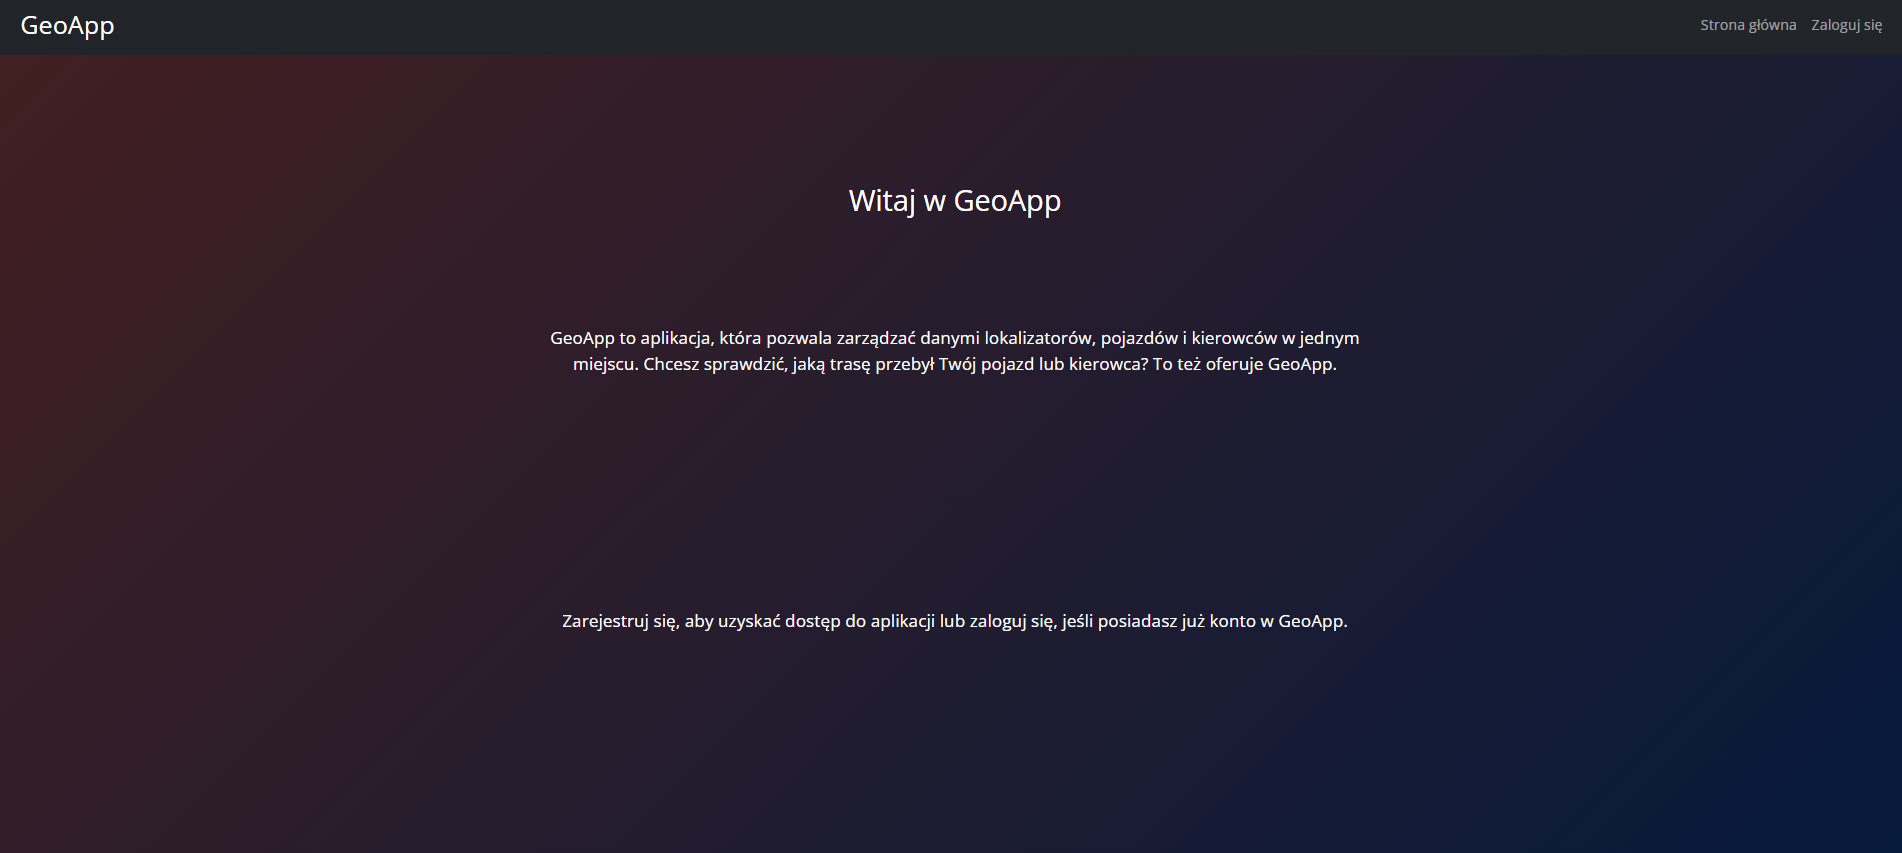
\includegraphics[width=1\textwidth]{./graf/home_page.png}
	\caption{Zrzut ekranu przedstawiający stronę główną.}
	\label{fig:home_page}
\end{figure}

\paragraph{}
W pierwszej kolejności ukazuje się formularz logowania (rys. \ref{fig:login_form}). Jest to celowy zabieg, ponieważ użytkownik, po założeniu konta, z każdym kolejnym uruchomieniem aplikacji będzie się logował. Wynika z tego, iż liczba logowań będzie wyższa niż liczba rejestracji, a zatem będzie to częstsza operacja wykonywana przez użytkowników. W celu otwarcia formularza rejestracji, należy kliknąć w tekst w lewym dolnym rogu formularza logowania. Jego treść brzmi: „Nie masz jeszcze konta? Zarejestruj się” - rys. \ref{fig:login_form}. Jest to link, który umożliwia zmianę formularza z opcji do zalogowania się, na opcję do utworzenia konta. Aby stworzyć konto użytkownika, należy wpisać adres email, z którym będzie owe konto powiązane. Kolejnym etapem jest ustalenie hasła, którym następnie wypełnia się drugie pole. W celach bezpieczeństwa, hasło powinno być trudne do rozszyfrowania przez innych ludzi. Niemniej jednak, nie ma możliwości odzyskania zapomnianego hasła, o czym warto pamiętać podczas korzystania z aplikacji. Aby dokończyć proces tworzenia konta, należy nacisnąć niebieski przycisk w prawym dolnym rogu. Widok formularza rejestracji znajduje się na rys. \ref{fig:register_form}.

\begin{figure}
	\centering
	
\includegraphics[width=0.6\textwidth]{./graf/login_form.png}
	\caption{Zrzut ekranu przedstawiający formularz logowania.}
	\label{fig:login_form}
\end{figure}

\begin{figure}
	\centering
	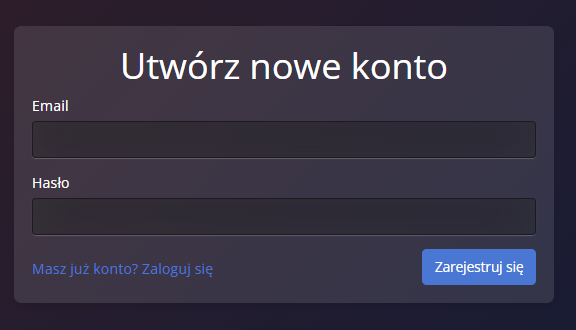
\includegraphics[width=0.6\textwidth]{./graf/register_form.png}
	\caption{Zrzut ekranu przedstawiający formularz rejestracji.}
	\label{fig:register_form}
\end{figure}

\paragraph{}
Do formularza logowania można dostać się na dwa sposoby. Jeden został wymieniony powyżej, drugim jest kliknięcie w tekst znajdujący się w lewym dolnym narożniku formularza rejestracji, brzmiący: „Masz już konto? Zaloguj się”. Dzięki temu w prosty sposób można przejść do zalogowania się, bezpośrednio po stworzeniu konta. Formularz logowania zawiera dwa pola, jedno służy do wpisania adresu email, z którym powiązane jest konto. W drugie pole należy wpisać hasło, które zostało ustalone podczas rejestracji. Zamiast znaków wpisywanych w to pole, pojawiają się kropki. Jest to mechanizm służący podniesieniu bezpieczeństwa, aby żadna dodatkowa osoba będąca w bliskiej okolicy użytkownika nie była w stanie przeczytać hasła, które jest wprowadzane. Po wypełnieniu obydwu pól wystarczy kliknąć niebieski przycisk pod formularzem.

\paragraph{}
W przypadku poprawnego wprowadzenia emailu oraz hasła, na ekranie ukazuje się panel użytkownika (rys.\ref{fig:user_tab}). Służy on przede wszystkim do dodawania powiązań między kierowcami, pojazdami i lokalizatorami, natomiast w pierwszej kolejności trzeba dodać poszczególne obiekty, jakimi są kierowca, pojazd czy lokalizator. Niemniej jednak, założono, że w trakcie używania aplikacji, użytkownicy nie często będą dodawać np. nowe pojazdy, stąd pierwszą zakładką, jaka pokazuje się po zalogowaniu, jest panel użytkownika. 

\begin{figure}
	\centering
	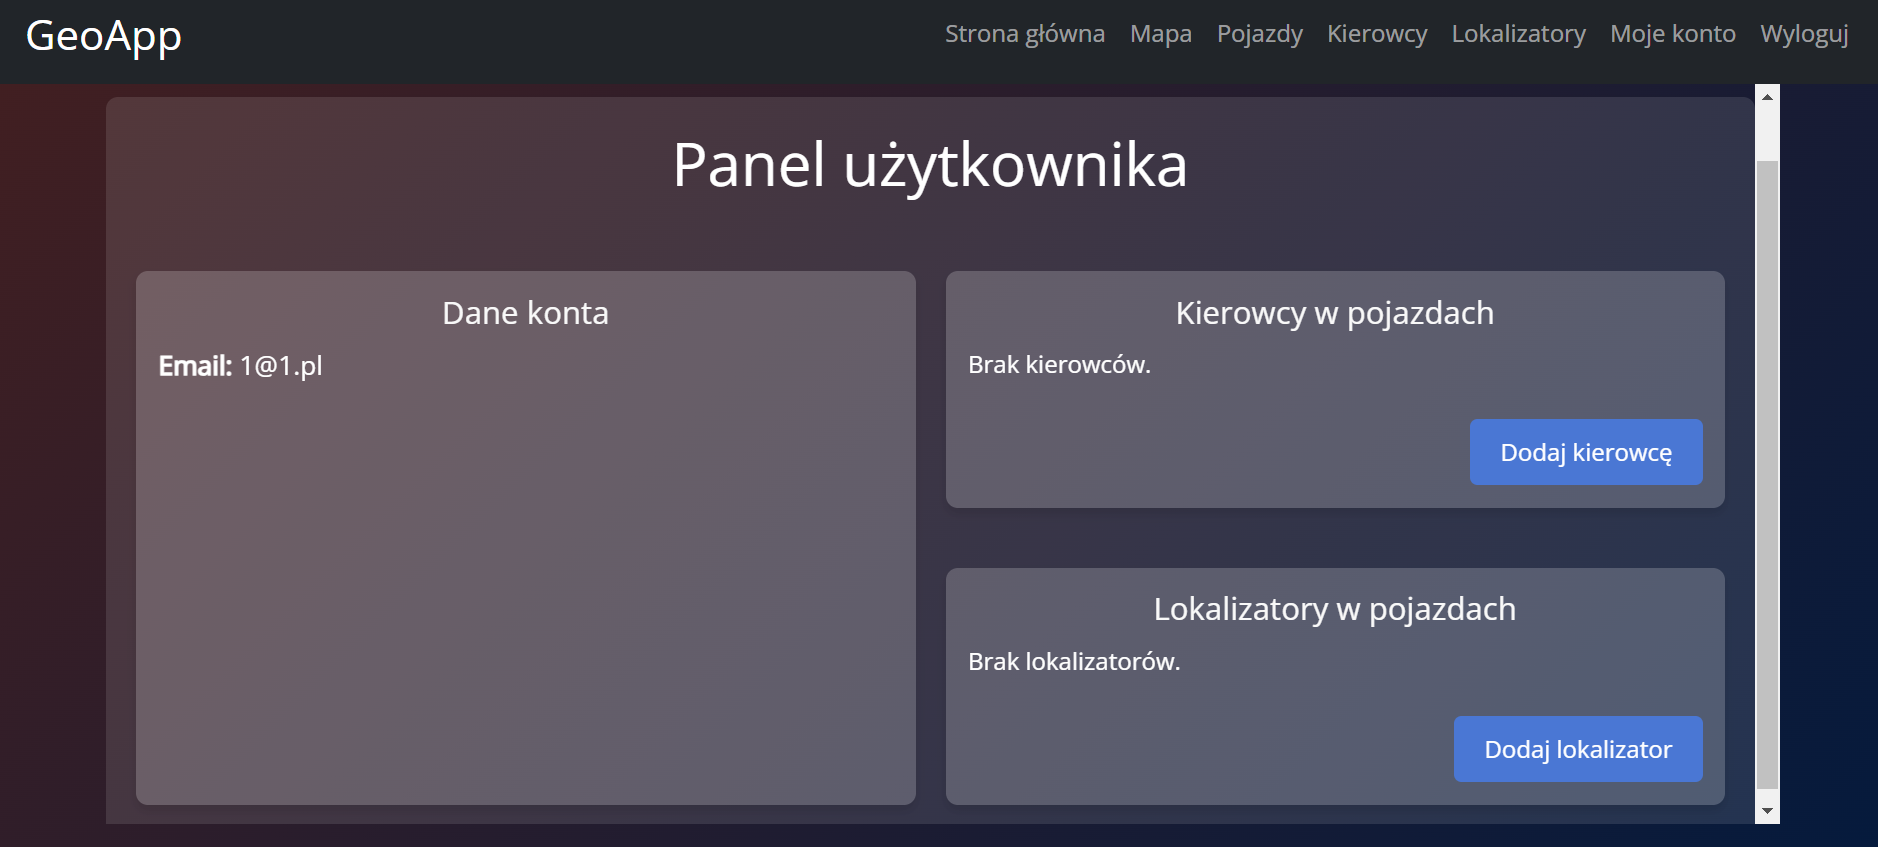
\includegraphics[width=0.6\textwidth]{./graf/user_tab.png}
	\caption{Zrzut ekranu przedstawiający zakładkę Moje konto.}
	\label{fig:user_tab}
\end{figure}


\paragraph{}
Aby dodać kierowcę, w pierwszej kolejności należy przejść do zakładki nazwanej „Kierowcy”. Podstawowym elementem tej części aplikacji jest lista kierowców. W przypadku gdy lista jest pusta, wyświetlany jest tekst „Brak kierowców.”, widoczny na rys. \ref{fig:driver_tab}. Pod listą lub napisem świadczącym o pustej liście znajduje się przycisk służący do dodania nowego kierowcy do listy. Po naciśnięciu przycisku otworzy się formularz - jego wygląd jest dostępny na rys. \ref{fig:add_driver}. Należy wypełnić jego pola, którymi są imię oraz nazwisko kierowcy. Przycisk oznaczony napisem „Dodaj kierowcę” pozwala dokończyć proces i zapisać wprowadzone dane w systemie. Formularz zostanie zamknięty, a na liście pojawi się nowa pozycja - przykład widoku z przykładowym kierowcą przedstawia rys. \ref{fig:driver_tab_2}. W przypadku kliknięcia czerwonego przycisku „Anuluj”, proces dodawania kierowcy zostanie wycofany, a aplikacja wróci do widoku zakładki z listą kierowców. Będąc tej w zakładce, użytkownik ma również możliwość usunięcia wybranego kierowcy. Służy do tego przycisk „Usuń”, znajdujący się po prawej stronie od każdej pozycji na liście.

\begin{figure}
	\centering
	
\includegraphics[width=0.6\textwidth]{./graf/driver_tab.png}
	\caption{Zrzut ekranu przedstawiający zakładkę Kierowcy.}
	\label{fig:driver_tab}
\end{figure}

\begin{figure}
	\centering
	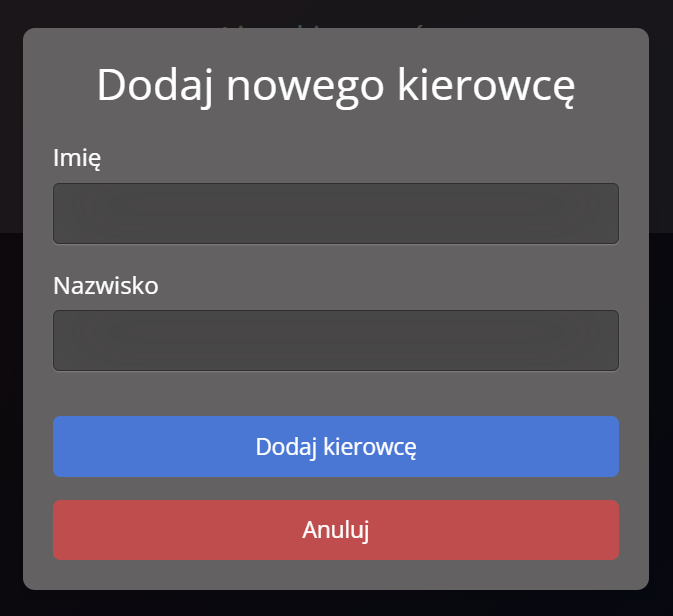
\includegraphics[width=0.6\textwidth]{./graf/add_driver.png}
	\caption{Zrzut ekranu przedstawiający formularz dodawania kierowcy.}
	\label{fig:add_driver}
\end{figure}

\begin{figure}
	\centering
	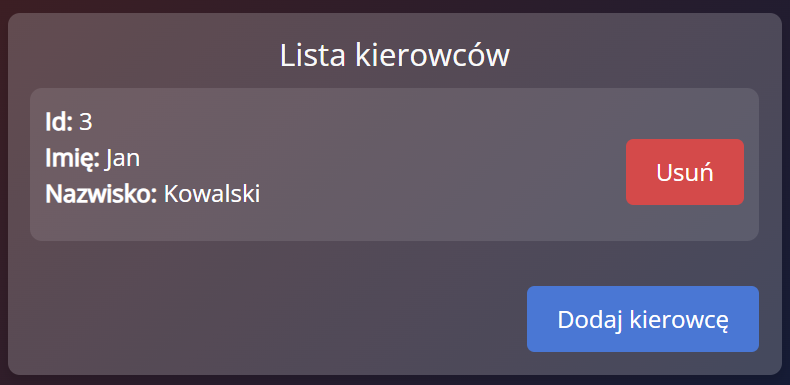
\includegraphics[width=0.6\textwidth]{./graf/driver_tab_2.png}
	\caption{Zrzut ekranu przedstawiający zakładkę Kierowcy z jednym kierowcą na liście.}
	\label{fig:driver_tab_2}
\end{figure}

\paragraph{}
Zakładką o analogicznym działaniu jest zakładka „Pojazdy”. Posiada listę samochodów zalogowanego użytkownika oraz przycisk pozwalający dodać do niej nową pozycję - wygląd z pustą listą znajduje się na rys. \ref{fig:vehicle_tab}. Formularz w tym przypadku posiada cztery pola: marka, model, tablica rejestracyjna oraz VIN. Pierwsze dwa służą przede wszystkim zwiększeniu przejrzystości listy dla użytkownika, natomiast trzecie i czwarte pole umożliwiają rozróżnienie poszczególnych samochodów, podczas gdy są one tej samej marki oraz tego samego modelu. Rys. \ref{fig:add_vehicle} przedstawia formularz dodawania pojazdu. Usuwanie elementów z listy jest dostępne również za pomocą przycisku znajdującego się po prawej stronie od każdego pojazdu.

\begin{figure}
	\centering
	
\includegraphics[width=0.6\textwidth]{./graf/vehicle_tab.png}
	\caption{Zrzut ekranu przedstawiający zakładkę Pojazdy.}
	\label{fig:vehicle_tab}
\end{figure}

\begin{figure}
	\centering
	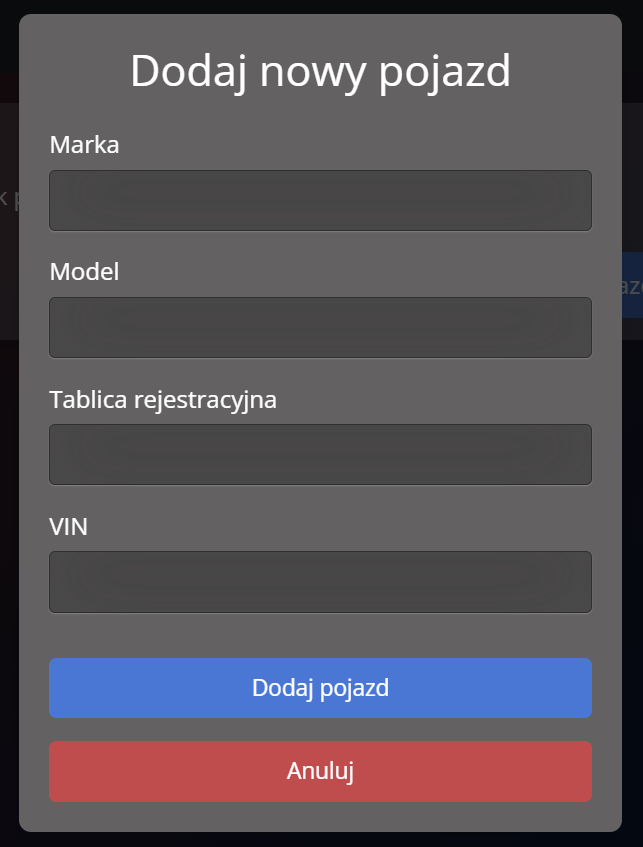
\includegraphics[width=0.6\textwidth]{./graf/add_vehicle.png}
	\caption{Zrzut ekranu przedstawiający formularz dodawania pojazdu.}
	\label{fig:add_vehicle}
\end{figure}

\paragraph{}
„Lokalizatory” to trzecia zakładka o podobnej zasadzie działania. Zrzut ekranu z jej wyglądem jest dostępny na rys. \ref{fig:tracker_tab}. Lista zawiera lokalizatory dodane przez użytkownika. Po kliknięciu w przycisk zatytułowany „Dodaj lokalizator”, otworzy się formularz, tym razem posiadający trzy pola do wypełnienia (rys.\ref{fig:add_tracker}). Nazwa jest dowolai, ma na celu ułatwić użytkownikowi znalezienie pożądanego lokalizatora na liście, numer seryjny jest polem identyfikacyjnym, które jest niepowtarzalne dla każdego urządzenia, natomiast w pole typ należy wpisać model urządzenia. W tym formularzu pojawia się również dodatkowy przycisk z napisem "Instrukcja - konfiguracja lokalizatora". Otwiera on dodatkowe okno z punktami, które trzeba wykonać, aby skonfigurować urządzenie do działania z aplikacją (rys. \ref{fig:help_dialog}). Można je zamknąć przyciskiem "Anuluj". Usuwanie odbywa się za pomocą przycisku „Usuń”, widocznego na rys. \ref{fig:tracker_tab}.

\begin{figure}
	\centering
	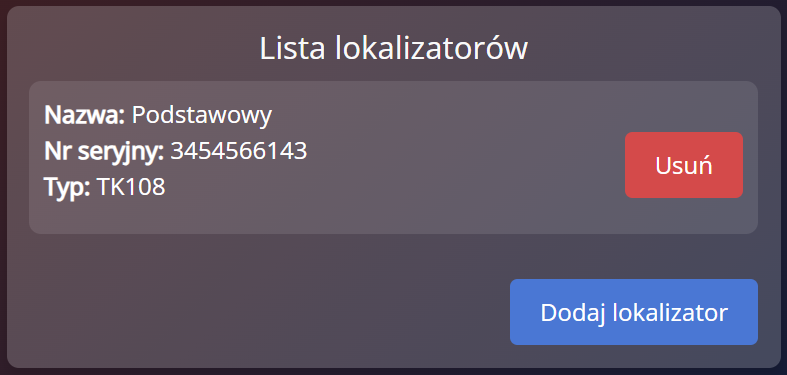
\includegraphics[width=0.6\textwidth]{./graf/tracker_tab.png}
	\caption{Zrzut ekranu przedstawiający zakładkę Lokalizatory.}
	\label{fig:tracker_tab}
\end{figure}

\begin{figure}
	\centering
	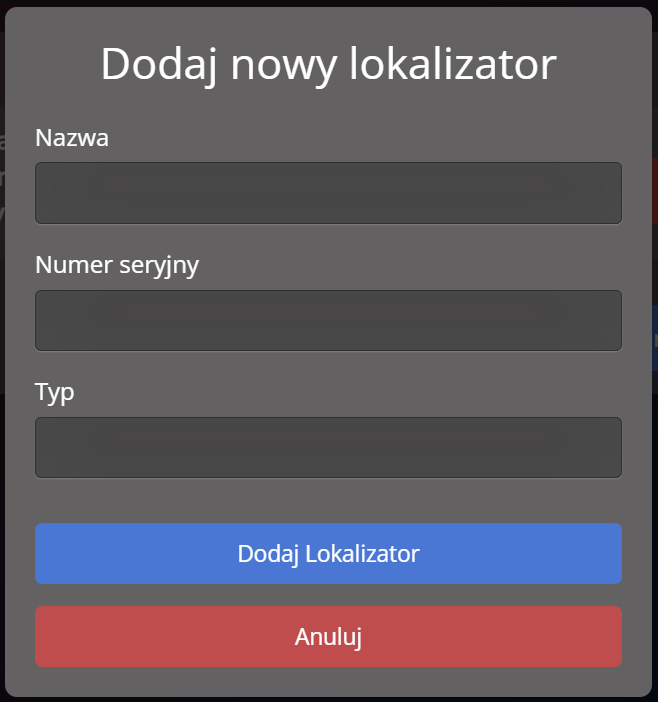
\includegraphics[width=0.6\textwidth]{./graf/add_tracker.png}
	\caption{Zrzut ekranu przedstawiający formularz dodawania lokalizatora.}
	\label{fig:add_tracker}
\end{figure}

\begin{figure}
	\centering
	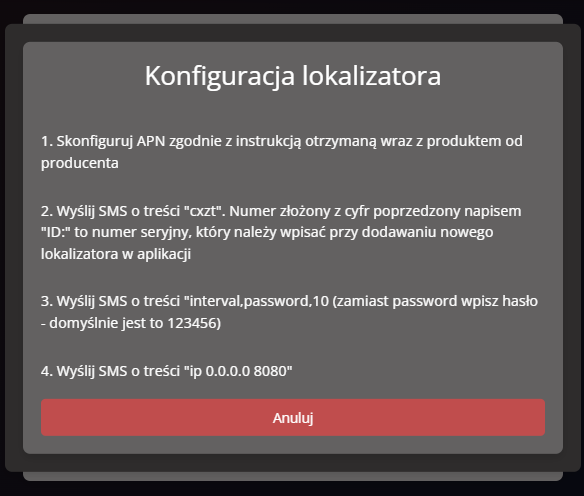
\includegraphics[width=0.6\textwidth]{./graf/help_dialog.png}
	\caption{Zrzut ekranu przedstawiający formularz dodawania lokalizatora.}
	\label{fig:help_dialog}
\end{figure}

\paragraph{}
Po dodaniu kierowców, pojazdów i lokalizatorów można przejść do tworzenia powiązań między nimi. W tym celu należy otworzyć zakładkę „Moje konto”, która przedstawia panel użytkownika. Aplikacja pozwala na stworzenie dwóch rodzajów powiązań:

\begin{itemize}
	\item kierowca pojazdu
	\item lokalizator w pojeździe
\end{itemize}

\paragraph{}
Kierowcy pojazdów, będący jednocześnie tytułem pierwszej listy w panelu użytkownika, definiują w jakim okresie czasu dany kierowca korzysta z danego pojazdu. Będzie to miało szczególne znaczenie podczas wyświetlania tras przebytych przez poszczególną osobę. W celu dodania powiązania, należy kliknąć przycisk „Dodaj kierowcę” (\ref{fig:user_tab}). Aplikacja wyświetli formularz składający się z czterech pól (rys. \ref{fig:add_driver_vehicle}). Pierwsze dwa są polami rozwijanymi, elementami pierwszego będą wszystkie pojazdy użytkownika, natomiast w drugim znajdować się będą jego kierowcy. Kolejne dwa pola to początek i koniec okresu użytkowania wybranego samochodu przez wybraną osobę. W celu wyznaczenia dat należy wybrać odpowiedni dzień z wyświetlonego kalendarza. Aby dokończyć proces tworzenia powiązania, należy kliknąć przycisk z napisem „Dodaj powiązanie”. Powiązanie zostanie zapisane do bazy danych i wyświetli się jako nowy element listy. Przycisk „Anuluj” czyści pola formularza jednocześnie go zamykając.

\begin{figure}
	\centering
	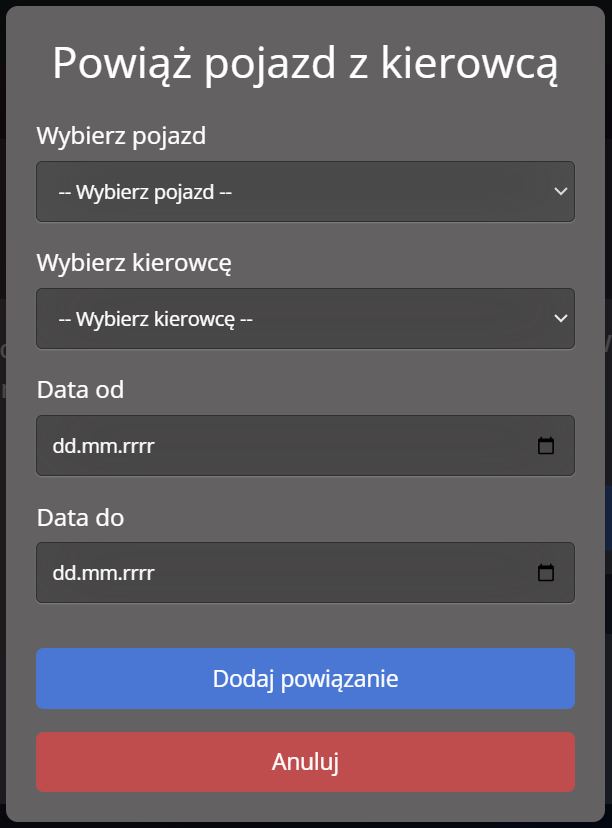
\includegraphics[width=0.6\textwidth]{./graf/add_driver_vehicle.png}
	\caption{Zrzut ekranu przedstawiający formularz dodawania powiązania kierowcy z pojazdem.}
	\label{fig:add_driver_vehicle}
\end{figure}


\paragraph{}
Drugą opcją powiązań są lokalizatory w pojazdach. Ich lista znajduje się pod listą kierowców pojazdów. Podobnie jak w przypadku pierwszego powiązania, formularz, który pozwala na dodanie nowego elementu od listy, ma cztery pola. Pierwsze pole jest niezmienione, co można zobaczyć na rys. \ref{fig:add_tracker_vehicle}. Jest to spowodowane faktem, iż to powiązanie również wykorzystuje pojazdy, zatem można w tym miejscu dokonać wyboru samochodu. Drugie pole uległo zmianie, jest to rozwijana lista lokalizatorów, z których należy wybrać jeden, który w danym okresie użytkownik planuje umieścić w pojeździe. Okres powiązania definiują kolejne dwa pola formularza, które również nie różnią się od pól wypełnianych podczas dodawania powiązania kierowcy z pojazdem. Przyciski oraz ich działanie jest także analogiczne do powyżej opisanego powiązania.

\begin{figure}
	\centering
	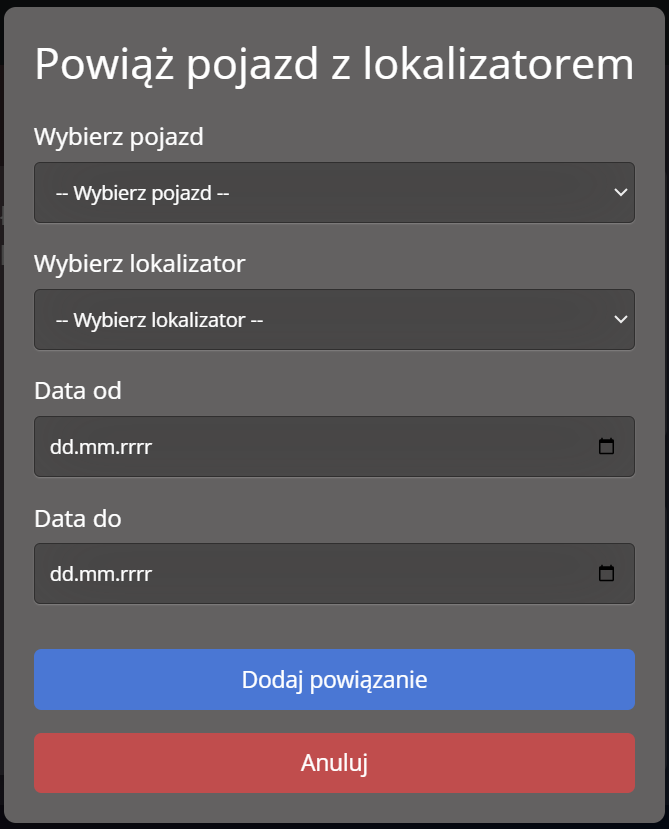
\includegraphics[width=0.6\textwidth]{./graf/add_tracker_vehicle.png}
	\caption{Zrzut ekranu przedstawiający formularz dodawania powiązania lokalizatora z pojazdem.}
	\label{fig:add_tracker_vehicle}
\end{figure}

\paragraph{}
Usuwania powiązań dokonuje się w identyczny sposób, w jaki zostało opisane usuwanie pojedynczych obiektów. Niemniej jednak, ważnym aspektem usuwania kierowców, pojazdów i lokalizatorów jest fakt, iż w przypadku uczestnictwa danego obiektu w jakimkolwiek powiązaniu, niedozwolone jest jego usunięcie. Pierwszym krokiem jest wtedy wyeliminowanie powiązania, z którym związany jest wybrany przez użytkownika np. kierowca, a następnie przeprowadzenie procesu usunięcia kierowcy.

\begin{figure}
	\centering
	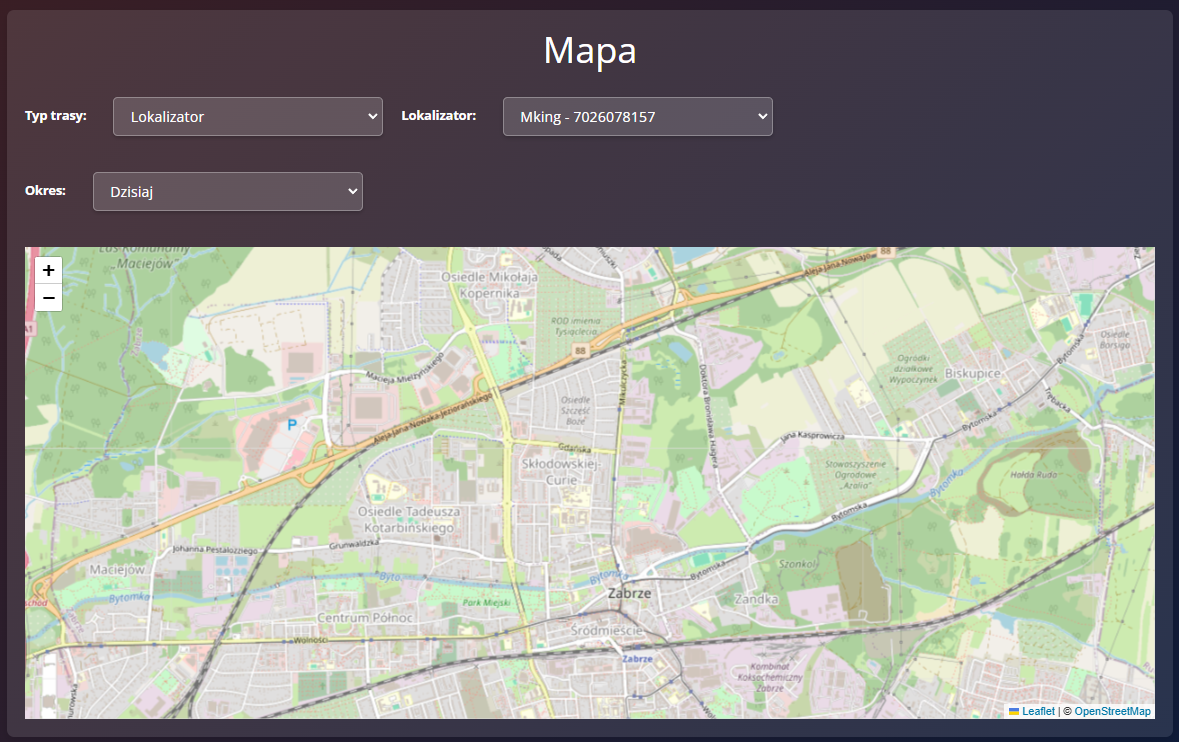
\includegraphics[width=0.6\textwidth]{./graf/map_tab.png}
	\caption{Zrzut ekranu przedstawiający zakładkę Mapa.}
	\label{fig:map_tab}
\end{figure}

\paragraph{}
Zakładka pod tytułem „Mapa” pozwala na wyświetlenie trasy z danego okresu czasu. Po jej otwarciu oczom użytkownika ukazuje się widok z rys. \ref{fig:map_tab}. Mapę można oddalać oraz przybliżać, korzystając z kółka myszy, a także przesuwać, poruszając myszą przy wciśniętym lewym przycisku. Pierwszą trasą, która wyświetla się po otwarciu zakładki jest trasa pierwszego z listy lokalizatora z bieżącego dnia, oczywiście w przypadku gdy ten lokalizator wysyłał dane na serwer tego dnia, to znaczy nie był wyłączony, rozładowany oraz został poprawnie skonfigurowany. Rozwijana lista nazwana "Lokalizator" pozwala wybrać konkretne urządzenie, którego trasę chcemy zobaczyć na mapie (rys. \ref{fig:/map_tracker}). Aby zmienić trasę na kierowcę lub pojazd, należy rozwinąć pole opisane jako "Typ trasy". Można wybrać wtedy opcję z listy, co widać na rys. \ref{fig:map_type}. W zależności od wybranego typu, rozwijana lista oznaczona słowem "Lokalizator" zmienia się w listę wyboru kierowcy lub pojazdu. Ostatnią opcją do wyboru jest "Okres", czyli dzień lub zakres dat, z którego chcemy wyświetlić trasę. Zgodnie z tym, co znajduje się na rys. \ref{fig:map_period}, można wybrać jedną z paru opcji domyślnych lub opcję "Niestandardowy", której kliknięcie skutkuje pojawieniem się dodatkowych dwóch pól (rys. \ref{fig:map_period}), w celu określenia daty początkowej i końcowej okresu do wyświetlenia trasy. Przykład ukazujący wygląd losowej trasy przedstawia rys. \ref{fig:map_route}.

\begin{figure}
	\centering
	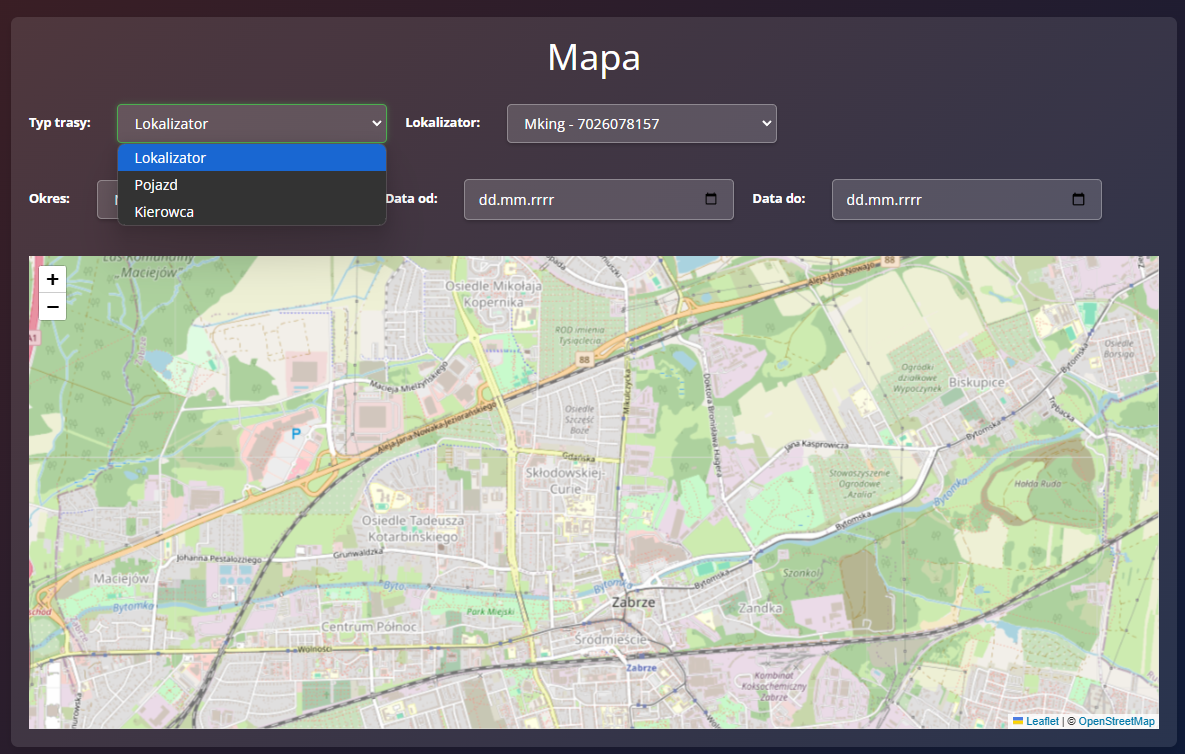
\includegraphics[width=1\textwidth]{./graf/map_type.png}
	\caption{Zrzut ekranu przedstawiający formularz dodawania trasy kierowcy.}
	\label{fig:map_type}
\end{figure}

\begin{figure}
	\centering
	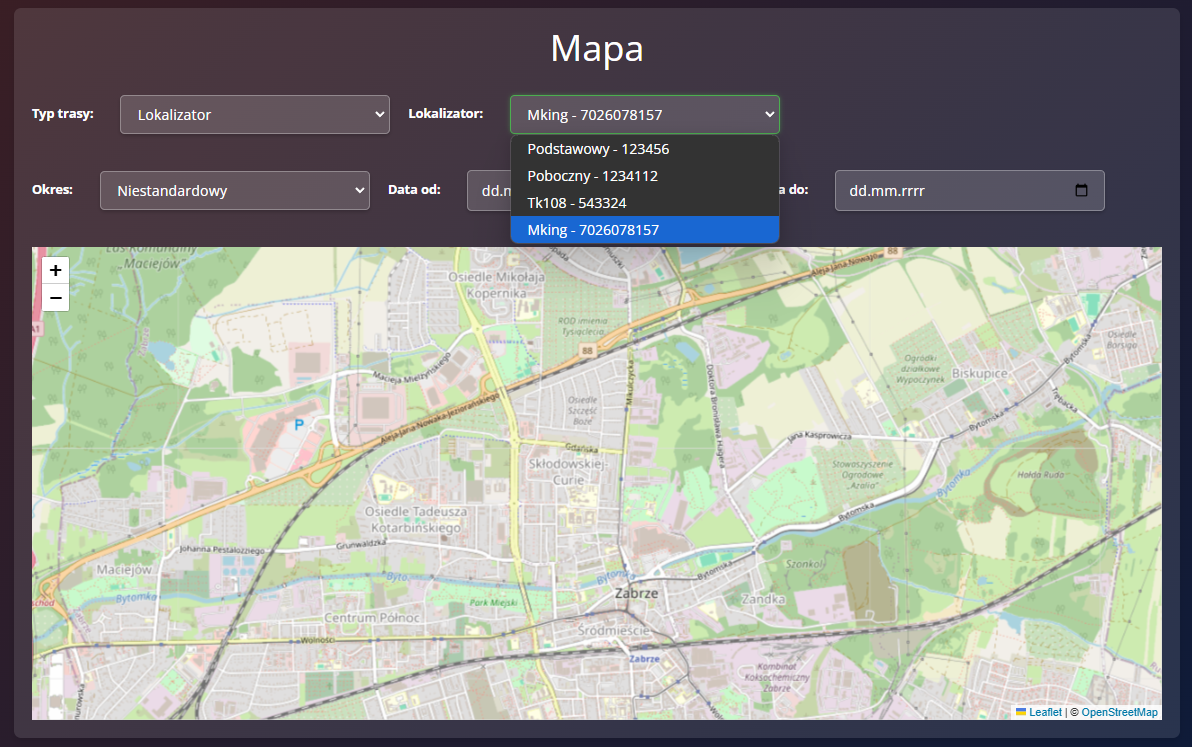
\includegraphics[width=1\textwidth]{./graf/map_tracker.png}
	\caption{Zrzut ekranu przedstawiający formularz dodawania trasy pojazdu.}
	\label{fig:/map_tracker}
\end{figure}

\begin{figure}
	\centering
	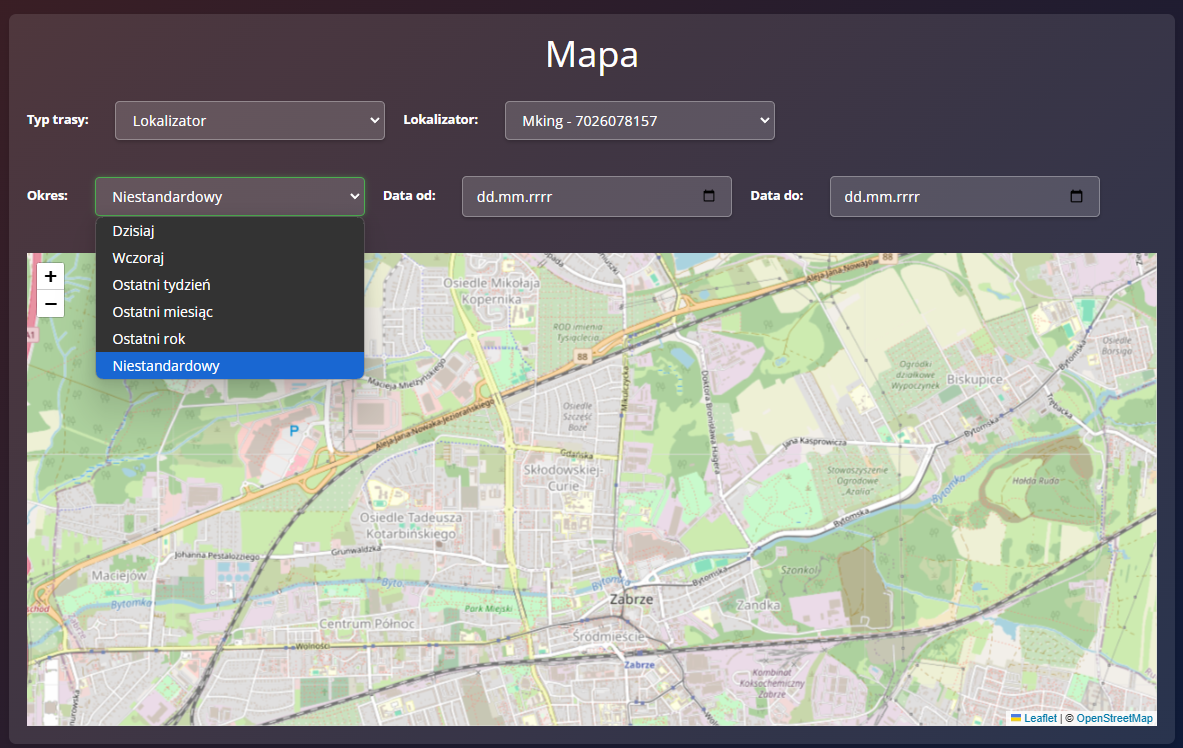
\includegraphics[width=1\textwidth]{./graf/map_period.png}
	\caption{Zrzut ekranu przedstawiający mapę z jedną trasą.}
	\label{fig:map_period}
\end{figure}

\begin{figure}
	\centering
	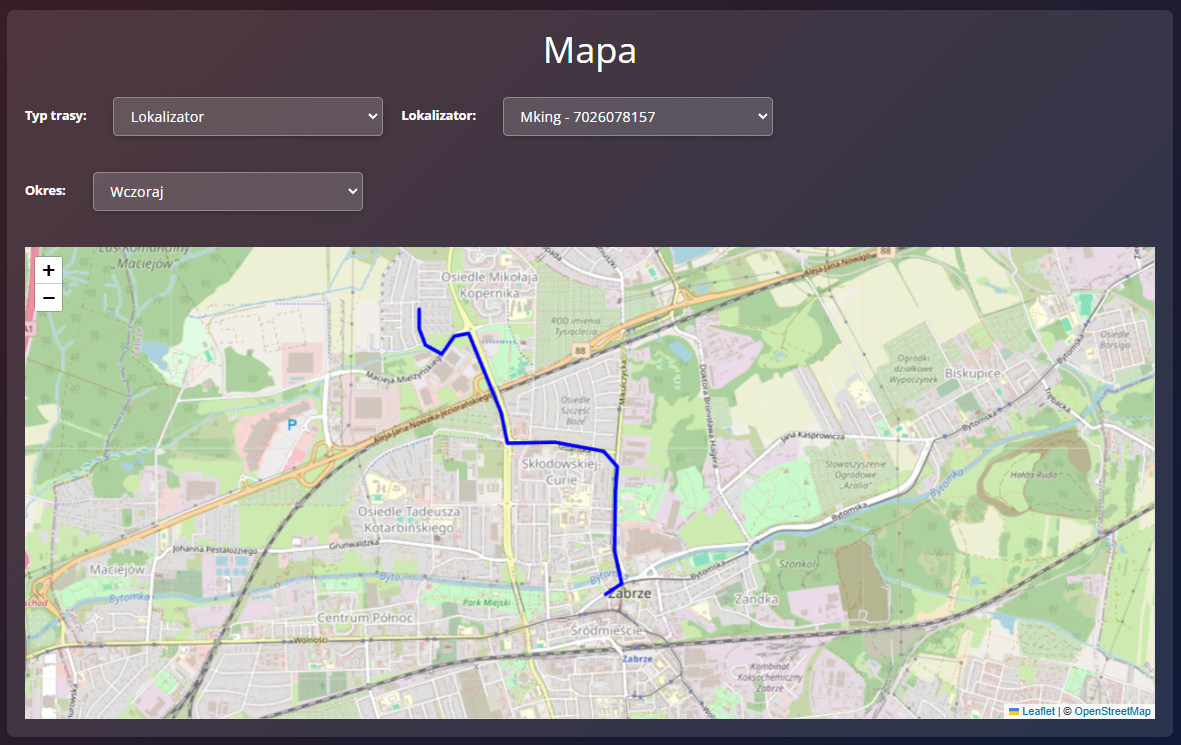
\includegraphics[width=1\textwidth]{./graf/map_route.png}
	\caption{Zrzut ekranu przedstawiający mapę z jedną trasą.}
	\label{fig:map_route}
\end{figure}


\paragraph{}
Na pasku nawigacyjnym zalogowanego użytkownika widnieje jeszcze jedna zakładka - „Wyloguj się” (rys. \ref{fig:user_tab}). Jest to tak naprawdę przycisk umożliwiający wylogowanie się z konta uzytkownika. Po jego kliknięciu, aplikacja nas wylogowuje i przenosi do strony głównej. Pojawia się wtedy pasek nawigacji widoczny na rys. \ref{fig:home_page}, co sprawia, iż w celu dostępu do funkcji zalogowanego użytkownika, należy ponownie się zalogować zgodnie z wyżej opisanymi krokami.

